% !TeX encoding = utf8
% !TeX spellcheck = fr

\chapter{Navigation}\label{cha:navigation}
Ce chapitre décrit le fonctionnement de la carte mobile en tant qu'aide à la navigation.
Il décrit les interactions possibles avec la carte et les informations de navigation qui peuvent y être superposées.

\begin{framed}
	\begin{center}
		\xc{} est entièrement développé par des bénévoles.\\
		Cette documentation aussi.\\
		Si vous y voyez des imperfections, vous pouvez facilement les faire disparaître~:\\
		\xcsoarwebsite{/develop/}
	\end{center}
\end{framed}

\section{Éléments de la carte mobile}

\begin{maxipage}
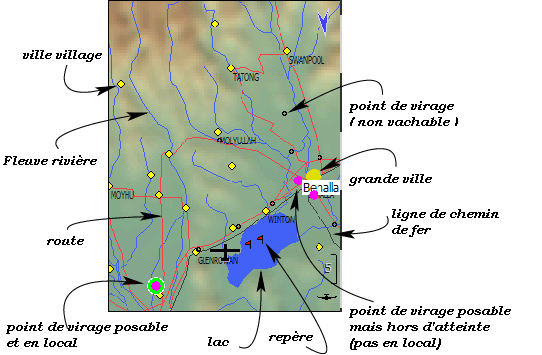
\includegraphics[angle=0,width=0.9\linewidth,keepaspectratio='true']{figures/fig-map.png}
\end{maxipage}

Peuvent être représentés sur la carte~:
\begin{enumerate} 
\item Planeur, vent, profil du thermique, indicateur d'arrivée
\item Terrain, relief et altitude du terrain
\item Topographie, rivières, routes, agglomérations
\item Points de virage, aérodromes, terrains posables
\item Le circuit en cours, zones d'observation, points de virage
\item Le cap à suivre (ou route à suivre\footnote{Direction menant au prochain point de virage~: la \emph{route}, voir paragraphe~\ref{sec:route}.}) 
\item Espaces aériens
\item Repères, historique des thermiques, trace au sol
\item Zone atteignable en plané\footnote{La zone atteignable en plané est aussi nommée \emph{local}, comme décrit dans le paragraphe~\ref{sec:reach}.}
\end{enumerate}
La carte est représentée dans un système de coordonnées projetées (pas en latitude et longitude), l'échelle est modifiable (zoom, dézoom) et la carte peut être déplacée dans toutes les directions. Toutes les fonctionnalités de navigation prennent en compte la courbure de la Terre.

\section{Symbole du planeur, orientation de la carte}
Le symbole du planeur montre sa position sur la carte. L'orientation du planeur indique le cap estimé du planeur.

La carte peut être orientée de trois façons~: 
\begin{enumerate}
\item Nord en haut
\item Route vers le haut
\item Objectif vers le haut
\end{enumerate}
Le paramétrage de l'orientation \config{orientation} permet de définir un autre mode d'orientation durant les spirales. Ceci est très utile pour ne pas être désorienté en regardant la carte en spirale. Le mode ``Objectif vers le haut'' en spirale facilite le choix de la direction à prendre lors de la sortie du thermique.

Quand les orientations ``Route vers le haut'' ou ``Objectif vers le haut'' sont utilisés en spirale, le symbole du planeur est au milieu de l'écran même si la position du symbole planeur a été configurée autrement.
En mode ``Transition'', les orientations ``Route vers le haut'' et ``Objectif vers le haut'' permettent de positionner le symbole du planeur à, par exemple, 20\% du bas de l'écran, donnant ainsi une bonne visualisation de la carte devant le planeur. Cette position par rapport au bord bas de l'écran est paramétrable dans le menu de
\config{gliderposition} configuration.

\section{Zoom et échelle de la carte}\label{sec:zooming}

Le changement d'échelle de la carte dépend de l'appareil~:
\begin{enumerate}
\item Appuyez/cliquez sur une partie neutre de la carte pour la sélectionner si elle ne l'est pas déjà.
Puis utilisez la roulette de la souris ou les flèches haut/bas du Pocket PC pour zoomer/dézoomer.
\item Les terminaux Android sont munis d'un bouton bascule permettant de changer d'échelle (il permet normalement de régler le volume). Situé sur le côté du terminal, il n'est guère accessible en vol lorsque l'appareil est dans un support générique.
\item Vous pouvez changer d'échelle d'un simple geste. Le geste  \gesture{Haut/Bas}
``Appui + Haut'' zoome, ``Appui + Bas'' dézoome.
\item Vous pouvez aussi sélectionner la fonction à l'aide des menus~:
\begin{quote}
\bmenug{Affich. 1}\blink\bmenug{Zoom} et \bmenug{Affich 1.}\blink\bmenug{Dézoom}
\end{quote}
\end{enumerate}

L'échelle est visible dans l'angle inférieur gauche de la carte mobile.
La distance indiquée est la distance sur la carte comprise entre les deux bords de l'écran.
\marginpar{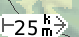
\includegraphics[angle=0,width=0.4\linewidth,keepaspectratio='true']{figures/zoom.png}}

Utilisateurs de Compaq Aero~: si vous activez les touches de jeux Compaq Aero (avec le Q-menu) les deux boutons centraux deviennent alors les touches Haut/Bas.

\subsection*{Zoom en mode spirale}
Deux paramétrages du zoom sont possibles~: l'un pour le vol en spirale et l'autre pour les modes ``Transition'' et ``Arrivée''.
C'est l'option ``Zoom en spirale'' dans le \config{circlingzoom} menu de configuration.
Par défaut, le ``Zoom en spirale'' est défini entre 2,5~km et 5~km en fonction de la taille de l'écran.
Quand l'utilisateur zoome/dézoome, ceci affecte uniquement le zoom du mode actuellement utilisé.
Ceci fait qu'en sortant de spirale, l'utilisateur retrouve l'échelle qu'il avait avant.
Si ``Zoom en spirale'' est sur ``off'', il n'y a alors qu'un seul niveau de zoom.
Cela conduit à gérer manuellement les différents niveaux de zoom à utiliser, indépendamment du paramétrage du zoom automatique (voir ci-dessous).

\subsection*{Zoom automatique}
Le zoom automatique permet de zoomer automatiquement à l'approche d'un point de virage, afin de garder celui-ci à l'écran. Quand \emph{Zoom Auto.} est actif, ``AUTO'' apparaît au-dessus de l'échelle actuelle dans l'angle inférieur gauche de l'écran. L'utilisateur peut toujours zoomer/dézoomer s'il le souhaite. Le contrôle du zoom passe alors automatiquement en mode Zoom Manuel.
\marginpar{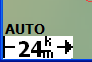
\includegraphics[angle=0,width=0.4\linewidth,keepaspectratio='true']{figures/zoomauto.png}}

Pour passer en mode \emph{Zoom Auto.}, utiliser le geste \gesturespec{ud}
ou le menu affiché à gauche. 
Revenir au zoom manuel se fait simplement en utilisant le même menu
ou en ajustant manuellement le zoom, que ce soit via le menu ou un geste.
\menulabel{\bmenug{Affich. 1}\blink\bmenut{Zoom}{Auto}}

Quand un point de virage change (automatiquement, à l'aide du gestionnaire de circuit ou par changement manuel du point de virage), \emph{Zoom auto.} règle automatiquement le niveau de zoom de l'affichage
afin de faire apparaître à l'écran le prochain point de virage.

En spirale, si une ascendance est détectée, alors la carte est centrée à proximité du thermique
tout en faisant en sorte que le planeur reste toujours visible.

\section{Déplacement de la carte}\label{sec:panning}

Le mode déplacement panoramique de la carte permet de se déplacer sur toute la carte tout en gardant la même échelle. Ceci est très utile lors de la préparation des circuits.
\begin{enumerate}
\menulabel{\bmenug{Affich. 1}\blink\bmenug{Panor. On}}
\item Activez le mode déplacement par le menu ou par geste. Le geste à faire est de déplacer votre doigt vers le haut, la droite, le bas puis la gauche, un peu comme un ``P''.
\gesturespec{urdl}
\item La carte peut alors être déplacée en tirant l'écran avec le doigt ou en utilisant les touches du curseur.
\item Le mode panoramique doit être désactivé manuellement, en utilisant ``\emph{Panor. Off}'' depuis le
sous-menu spécifique au mode panoramique.
\end{enumerate} 

\sketch{figures/pan.png}
Quand le mode panoramique est activé, ``PAN'' s'affiche au-dessus de l'échelle. 
Les coordonnées GPS affichées en haut et à droite sont celles de la petite croix du centre. Si la carte topographique est chargée, l'altitude du point est affichée.

La carte permet d'utiliser la fonction ``\emph{Qu'y a-t-il ici?}'' en appuyant simplement sur n'importe
quel endroit de la carte (avec un écran tactile).
Un menu spécifique apparaît alors, facilitant l'exploration de la carte et la préparation des circuits.

\section{Points de virage}\label{sec:waypoint-schemes}
Les points de virage sont représentés différemment suivant leur type, la principale caractéristique étant les points de virage ``posable'' ou ``non posable''.

\subsection*{Posables}
La représentation des points de virage est donnée ci-dessous. Il existe trois ensembles de symboles pour les points de virages posables~:\config{waypointicons}

\begin{tabular}{c|ccc|ccc|}
\begin{sideways}Ensemble de symboles\end{sideways}
&\begin{sideways}Champ posable\end{sideways}
&\begin{sideways}Limite\end{sideways}
&\begin{sideways}En local\end{sideways}
&\begin{sideways}Aérodrome\end{sideways}
&\begin{sideways}Limite\end{sideways}
&\begin{sideways}En local\end{sideways}\\
\hline
Cercle violet &

\includegraphics[width=0.8cm]{icons/winpilot_landable.pdf} &

\includegraphics[width=0.8cm]{icons/winpilot_marginal.pdf} &

\includegraphics[width=0.8cm]{icons/winpilot_reachable.pdf} &
\colorbox{white}{
\includegraphics[width=0.8cm]{icons/winpilot_landable.pdf}} &

\includegraphics[width=0.8cm]{icons/winpilot_marginal.pdf} &

\includegraphics[width=0.8cm]{icons/winpilot_reachable.pdf} \\
\hline
Noir et blanc & 

\includegraphics[width=0.9cm]{icons/alt_landable_field.pdf} &

\includegraphics[width=0.9cm]{icons/alt_marginal_field.pdf} &

\includegraphics[width=0.9cm]{icons/alt_reachable_field.pdf} &
\colorbox[rgb]{0.94,0.94,0.94}{
\includegraphics[width=0.9cm]{icons/alt_landable_airport.pdf}} &

\includegraphics[width=0.9cm]{icons/alt_marginal_airport.pdf} &

\includegraphics[width=0.9cm]{icons/alt_reachable_airport.pdf} \\
\hline
Feux tricolores & 

\includegraphics[width=0.9cm]{icons/alt2_landable_field.pdf} &

\includegraphics[width=0.9cm]{icons/alt2_marginal_field.pdf} &

\includegraphics[width=0.9cm]{icons/alt_reachable_field.pdf} &
\colorbox{white}{
\includegraphics[width=0.9cm]{icons/alt2_landable_airport.pdf}} &

\includegraphics[width=0.9cm]{icons/alt2_marginal_airport.pdf} &

\includegraphics[width=0.9cm]{icons/alt_reachable_airport.pdf} \\
\hline
\end{tabular}

Les symboles ``\emph{Limite}'' sont dessinés pour les points de virage qui sont en principe atteignables
en finesse, mais pour lesquels il n'est pas possible de réaliser une approche directe, comme
lorsqu'il y a un relief sur la route.
 
En option, les points de virage peuvent être étiquetés selon l'un des
schémas d'abréviation \config{labels} et leur visibilité.

En plus de cela, des détails supplémentaires peuvent être affichés à propos des points de virage posables.
Si
``\emph{Terrains posables détaillés}''
est activé, vous avez des informations en plus au travers de l'apparence du symbole~:
\begin{enumerate}
\item Les champs posables ont un symbole carré, contrairement à ce qui est présenté dans le tableau.
Le carré est dessiné comme un losange posé sur l'un de ses coins.
Les aérodromes conservent le symbole circulaire, de façon à être facilement différenciés.
\item Tous les ensembles de symboles, ``Cercle violet'' inclus, ont leurs pistes dirigées dans la direction réelle. Pour cela, la direction des axes de piste doit être renseignée dans la base de données des points de virage. Par exemple, le format de fichier de 
points de virage de SeeYou (\verb|.cup|) inclut cette information.
\end{enumerate}

\subsection*{Posables en local}
À proximité d'un point posable en local est affiché la hauteur
estimée d'arrivée \emph{au-dessus de la hauteur de sécurité en arrivée}.
Cette fonctionnalité est l'une des plus puissantes d'\xc.
La hauteur d'arrivée est calculée par ``\emph{le calculateur de vol}''
d'\xc{} en prenant en compte les paramètres de performance du planeur (polaire),
de calage du MacCready, de vent, de hauteur de survol
du relief (garde au sol), et --- évidemment --- des hauteurs de sécurité.
Tous ces paramètres étant configurables, il est facile de se tromper.
Aussi, s'il vous plaît~: à moins que vous ayez une compréhension approfondie des concepts du calculateur de vol, vous
\warning
feriez mieux de garder la pré-configuration d'\xc{} (et de ne pas prendre bêtement les valeurs calculées pour la ``Vérité révélée'').
C'est toujours au pilote d'interpréter les valeurs affichées et de suivre leurs évolutions au cours du temps.

Selon comment est configuré le calculateur de vol (chapitre~\ref{cha:glide}),
les hauteurs d'arrivée estimées, 
affichées à côté des points posables en local, pourraient prendre en compte le relief ou pas,
voire les deux pourraient être affichées.
\config{arrivalheight}

Une autre possibilité est d'afficher la finesse nécessaire à côté
du point posable en local. Ce calcul est simplement dérivé de la
distance réelle entre le planeur et le point posable,
divisée par la différence de hauteur entre l'altitude actuelle et
l'altitude du point posable. Là encore, la hauteur de sécurité
est ajoutée à l'altitude du point posable, mais rien d'autre
n'est pris en compte~: pas de vent, ni de polaire, ni de calage
MacCready. C'est juste un calcul géométrique.
Le concept de finesse nécessaire est encore très discuté,
bien qu'on dit qu'il soit très robuste.

\tip Garder à l'esprit la très forte relation entre les affichages de la \emph{distance atteignable} et le paramétrage du calculateur de vol.

\subsection*{Non-posables}
À condition que votre fichier de points de virage contienne des informations sur la nature
des points de virage non-posables, la carte les affichera avec des symboles spécifiques.
La figure~\ref{fig:nonlandables} contient une liste des symboles actuellement gérés par la carte.

\begin{figure}[htbp]
\centering
\vspace{2.5cm}
\begin{tabular}{ccccccccc}
\begin{rotate}{60}Point de virage simple\end{rotate} &
\begin{rotate}{60}Sommet de montagne\end{rotate} &
\begin{rotate}{60}Obstacle\end{rotate} &
\begin{rotate}{60}Col\end{rotate} &
\begin{rotate}{60}Centrale électrique\end{rotate} &
\begin{rotate}{60}Tour ou bâtiment\end{rotate} &
\begin{rotate}{60}Tunnel\end{rotate} &
\begin{rotate}{60}Station météo\end{rotate} &
\begin{rotate}{60}Pont\end{rotate}\\

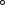
\includegraphics[width=0.5cm]{icons/map_turnpoint.pdf} &
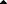
\includegraphics[width=0.8cm]{icons/map_mountain_top.pdf} &
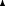
\includegraphics[width=0.7cm]{icons/map_obstacle.pdf} &
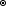
\includegraphics[width=0.7cm]{icons/map_pass.pdf} &
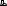
\includegraphics[width=0.8cm]{icons/map_power_plant.pdf} &
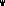
\includegraphics[width=0.7cm]{icons/map_tower.pdf} &
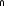
\includegraphics[width=0.6cm]{icons/map_tunnel.pdf} &
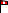
\includegraphics[width=0.6cm]{icons/map_weather_station.pdf} &
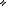
\includegraphics[width=0.8cm]{icons/map_bridge.pdf}
\end{tabular}
\caption{Points de virage non-posables}\label{fig:nonlandables}
\end{figure}

\section{Circuit en cours}

Le tracé du circuit en cours est représenté sur la carte par une ligne bleue pointillée.
Les secteurs et les aires des points de virage sont représentés par une surface surlignée en jaune.
Des cercles sont toujours représentés autour des points de départ et d'arrivée~;
des lignes y sont dessinées uniquement si ces points sont de type ligne.

Une ligne noire épaisse est affichée en permanence du planeur vers le prochain point de virage du circuit en cours.
Cette ligne peut pointer directement vers le point de virage, ou bien donner la trace d'un chemin contournant
relief et espaces aériens, comme décrit en détails dans le paragraphe~\ref{sec:route}.

\begin{center}
\begin{tabular}{c c c}
\emph{Départ/arrivée} & \emph{Secteur} & \emph{Cylindre} \\
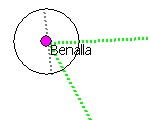
\includegraphics[angle=0,width=0.3\linewidth,keepaspectratio='true']{figures/cut-startfinish.png} &
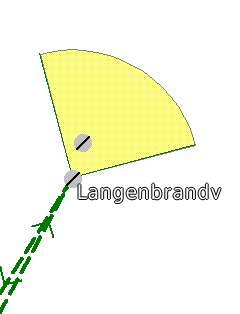
\includegraphics[angle=0,width=0.3\linewidth,keepaspectratio='true']{figures/cut-sector.png} &
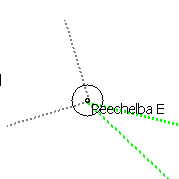
\includegraphics[angle=0,width=0.3\linewidth,keepaspectratio='true']{figures/cut-barrel.png}
\end{tabular}
\end{center}


\section{Relief et topographie}\label{sec:terrain_topo}

Les éléments topographiques affichés sur la carte sont~:
\begin{itemize}
\item Routes principales, sous forme de lignes rouges
\item Fleuves et rivières, sous forme de lignes bleues
\item Grandes étendues d'eau (lacs), zones bleues
\item Grandes villes, zones jaunes
\item Villages et petites villes, petits diamants jaunes
\end{itemize}
Les villes et villages sont écrits en italique.

Le relief est coloré en fonction de l'altitude et optionnellement ombré suivant la direction du soleil ou la direction du vent. Les reliefs non valides ou sous le niveau de la mer sont représentés en bleu.

\menulabel{\bmenug{Affich. 2}\blink\bmenut{Relief}{On/Off}}
\menulabel{\vspace{1cm}\bmenug{Affich. 2}\blink\bmenut{Topo.}{On/Off}}

Le relief est ombré pour améliorer sa lisibilité.
Par défaut, l'éclairage virtuel utilisé est celui du cap du vent estimé.
Ainsi, les faces les plus claires sont les faces portantes, les faces sombres sont sous le vent.
L'ombrage en fonction de la position du soleil est aussi implémentée.
Si l'ombrage des pentes est configuré pour ``Soleil'', les pentes les plus claires suivent l'heure de la journée de façon très naturelle.
L'ombrage et la clarté globales sont paramétrables. \config{shading}

L'affichage du relief et de la topographie peuvent être activés/désactivés par les menus.

\begin{center}
\begin{tabular}{c c}
Topographie & Relief \\
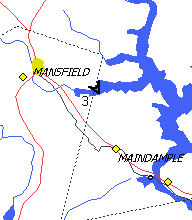
\includegraphics[angle=0,width=0.4\linewidth,keepaspectratio='true']{figures/cut-topo.png} &
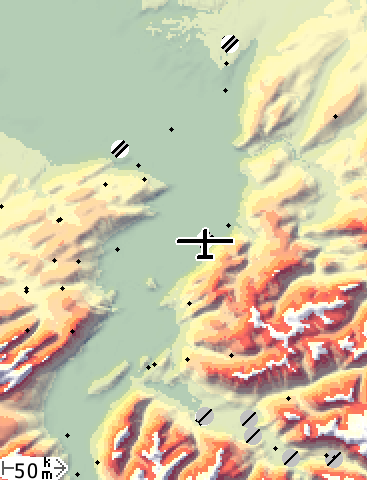
\includegraphics[angle=0,width=0.4\linewidth,keepaspectratio='true']{figures/cut-terrain.png}
\end{tabular}
\end{center}

Si la carte de relief n'est pas chargée (ou si son affichage est sur Off), le fond de la carte est blanc. Tout relief sous le niveau de la mer est représenté en bleu. Si vous volez en dehors de la carte ``relief'', le fond de carte sera aussi blanc.

\subsection*{Étiquettes sur la carte}\label{sec:maplabels}

L'écran peut contenir trop d'information et être peu lisible.
Il est alors possible de ne plus montrer les étiquettes des points de virage en modifiant le menu ``\emph{Étiquettes}''.
\menulabel{\bmenug{Affich. 2}\blink\bmenut{Étiquettes}{Aucun}} 

D'autres options pour diminuer l'encombrement de l'écran sont disponibles~:

\jindent{\bmenuth{Étiquettes}{Circuit \&}{Aérodromes}}{Affiche les noms des points de virage du
circuit en cours et de tous les aérodromes (basé sur les attributs des points de virages du
fichier de points de virage). Les autres points de virage sont représentés mais sans étiquette}
\jindent{\bmenut{Étiquettes}{Tous}}{Affiche les noms de tous les points de virage}
\jindent{\bmenuth{Étiquettes}{Circuit \&}{Terrains}}{Affiche les noms des points de virage du
circuit en cours et de tous les terrains posables (basé sur les attributs des points de virages du
fichier de points de virage). Les autres points de virage sont représentés mais sans étiquette}
\jindent{\bmenut{Étiquettes}{Circuit}}{Affiche uniquement les noms des points de virage du circuit en cours}

Dans tous les cas, le format des étiquettes reste paramétrable dans le menu de configuration ``\emph{Affichage de la carte / Points de virage}'. \config{labels}

\section{Trace sol}\label{sec:trail}

Une ``trace sol'' optionnelle est dessinée sur la carte et montre le trajet passé du planeur.
La couleur et l'épaisseur de la trace sont configurables en fonction de l'altitude ou de la valeur du variomètre.

\begin{center}
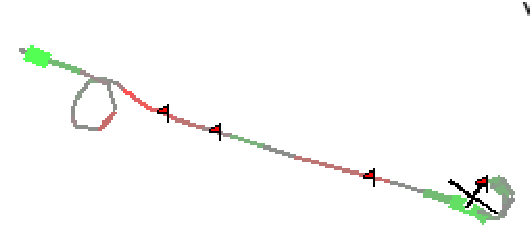
\includegraphics[angle=0,width=0.8\linewidth,keepaspectratio='true']{figures/snail.pdf}
\end{center}

Si un Vega ou un autre variomètre intelligent est connecté avec un sortie ``Netto'',
la valeur du vario Netto est utilisée. Alors la couleur et l'épaisseur de la trace sol
représentent la vitesse verticale de la masse d'air à la place de celle du planeur.

\config{snailtype}
La longueur de la trace sol peut être choisie entre \emph{Off}, \emph{courte} (environ 10~minutes),
\emph{longue} (environ une heure) ou encore \emph{complète} (depuis le début du vol).
Ce réglage peut être permanent en utilisant le menu de configuration \config{snailtrail} ou temporaire à l'aide du menu.
\menulabel{\bmenug{Affich. 2}\blink\bmenut{Trace}{Complet}} 

Quel que soit  le mode de trace choisi, en mode ``spirale'' la trace est courte afin de laisser la carte lisible.

Dans le but d'aider au centrage des ascendances quand il y a du vent, la trace sol en spirale
peut être compensée artificiellement en fonction du vent (dérive compensée en spirale).
De cette façon, la trace sol fait référence au vent et non plus au sol. Comme les thermiques
se déplacent aussi avec le vent, la trace sol compensée donne une meilleure
indication de la position du thermique par rapport au planeur.

La figure suivante en montre l'exemple. Quand la compensation de la dérive en spirale est activée
(figure de droite), le planeur semble tourner dans une colonne verticale plutôt que dans une colonne inclinée (figure de gauche).

\begin{center}
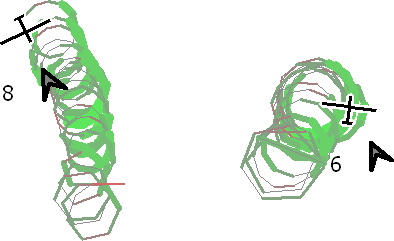
\includegraphics[angle=0,width=0.8\linewidth,keepaspectratio='true']{figures/traildrift.png}
\end{center}

\config{traildrift}
L'activation de la ``dérive compensée en spirale'' se fait dans le
menu de configuration du vent.  La compensation n'a lieu qu'en spirale~: la trace sol en transition n'en tient pas compte.
Le paramétrage peut se faire aussi avec fenêtre de configuration du vent.
\menulabel{\bmenug{Config. 1}\blink\bmenus{Vent}}

L'affichage de la dérive est aussi utile afin de montrer plus clairement
l'existence d'une inclinaison des thermiques due au cisaillement par le vent.

L'épaisseur de la trace sol peut être agrandie en fonction de la valeur du vario\config{trailscaled}.


\section{Marques}\label{sec:markers}

Les marques sont représentées par de petits drapeaux (a) sur la carte. Les marques peuvent être 
placées à la main en appuyant sur un bouton ou automatiquement. Un exemple d'utilisation
en mode automatique est de placer une marque à chaque entrée en mode ``spirale'', 
une façon simple de repérer tous les thermiques rencontrés.

\menulabel{\bmenug{Nav. 2}\blink\bmenug{Marquer}}
Les marques ne sont pas conservées sur la carte quand on éteint \xc.
Cependant, la position de toutes les marques est ajoutée au fichier \verb|xcsoar-marks.txt|.

\section{Marques de thermiques}

En montée dans les thermiques, des marques sont créées automatiquement et
affichées à l'écran. La position des 20~derniers thermiques est
stockée jusqu'à la fin du vol. 
\sketch{figures/thermalhistory.png}
Cette historique des thermiques est accessible par la
fonction ``Qu'y-a-t'il ici~?'', de la même façon que les autres marques et les points de virage.

En sélectionnant une marque sur la carte, vous obtenez la fenêtre suivante~:
\begin{center}
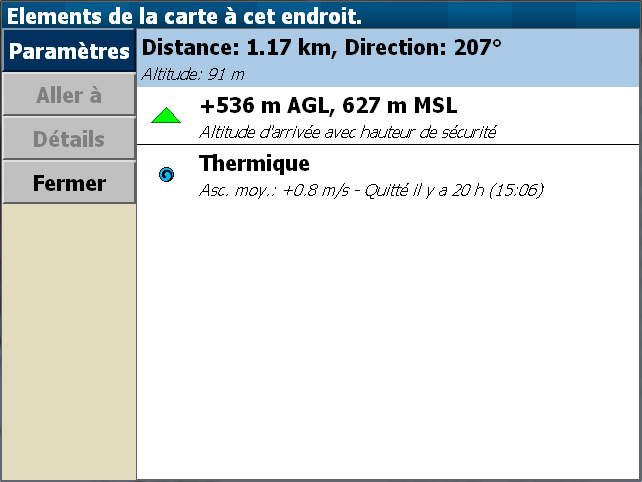
\includegraphics[angle=0,width=0.8\linewidth,keepaspectratio='true']{figures/marque_panel.png}
\end{center}

\section{Zone atteignable en plané}\label{sec:reach}

La limite de la zone atteignable en plané est représentée par
une ligne pointillée noire et blanche. Elle donne le contour de la zone
que peut atteindre le planeur avant d’arrivée à la hauteur minimale (hauteur d'arrivée).
La zone atteignable montre les trajectoires dans toutes les directions, avec possibilité de prendre en compte les trajectoires contournant
des reliefs. Cette fonctionnalité est utile pour estimer la rayon d'action
lorsque l'on est bas et que l'on recherche une ascendance, mais aussi lorsque l'on vole
en montagne.

Les calculs peuvent être configurés \config{turningreach} avec deux niveaux de détail~:
\begin{description}
\item[En ligne droite] Si le mode ``contournement'' est désactivé, alors la
zone atteignable montre la plus grande distance que le planeur peut parcourir en arrivée dans toutes les directions et en
ligne droite. La limite ressemble alors à une boucle fermée autour du planeur.

\begin{center}
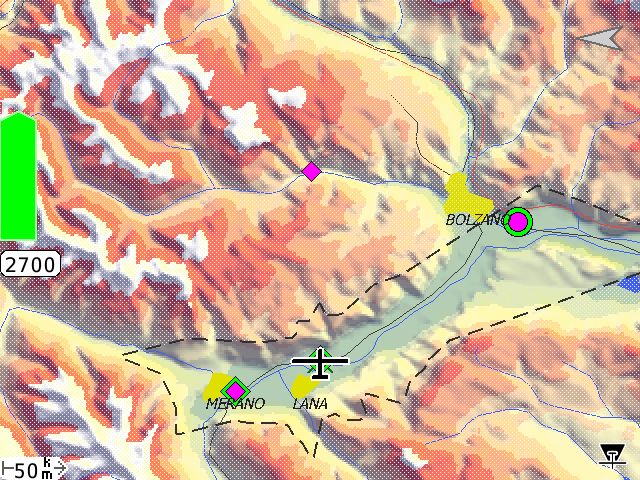
\includegraphics[angle=0,width=0.8\linewidth,keepaspectratio='true']{figures/reach1.png}
% CUTOUT SHOWING GLIDE RANGE FOOTPRINT.  NO TOPOGRAPHY, FULLSCREEN, NO TASK. TURNING=FALSE
\end{center}
 
\item[Contourne] Si le mode ``contournement'' est activé, alors la zone atteignable montre la 
plus grande distance que le planeur peut parcourir en arrivée dans toutes les directions, 
même en contournant des obstacles\footnote{Le nombre maximum de contournements est
de trois, et aucun contournement ne peut faire plus de 90°.}.  La
limite ressemble alors à une boucle fermée autour du planeur, mais peut aussi 
inclure des trous indiquant des sommets de montagne que le planeur ne peut pas atteindre
sans reprendre d'altitude.

\begin{center}
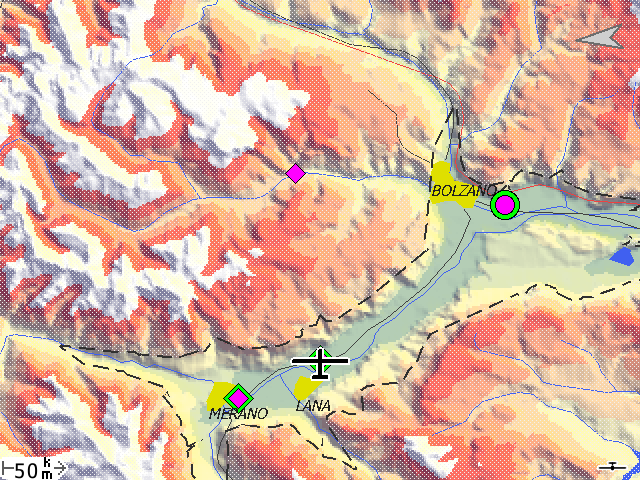
\includegraphics[angle=0,width=0.8\linewidth,keepaspectratio='true']{figures/reach2.png}
% CUTOUT SHOWING GLIDE RANGE FOOTPRINT.  NO TOPOGRAPHY, FULLSCREEN, NO TASK. TURNING=TRUE
\end{center}

\end{description}

L'affichage peut être configuré afin de rendre floue la zone
non atteignable. \config{gliderange}
La trajectoire d'arrivée prend en compte la hauteur du planeur au-dessus du relief
en considérant la garde au sol (voir paragraphe~\ref{sec:safety-heights}).
Si cette marge n'est pas conservée, une croix rouge apparaît sur la carte à l'endroit de la violation.
Si un objectif est sélectionné, le calcul est effectué en ligne droite vers cet objectif.
Si aucun objectif n'est sélectionné, le calcul est effectué avec le cap actuel.

Si ``zone atteignable en plané'' est activée, alors la possibilité d'atteindre des points
de virages posables est utilisée par le mode ``Abandon de circuit'', par la liste des ``dégagements'',
et par l'affichage des points de virage posables sur la carte.

Il faut noter que les calculs du circuit en cours ne sont pas impactés par les calculs de zone atteignable en plané.
Par exemple, la flèche d'altitude nécessaire dans la flèche d'arrivée
ou les données du circuit affichées dans les InfoBoxes ne prennent pas en compte la ``zone atteignable en plané''.

Les calculs de ``zone atteignable en plané'' sont utilisés pour la trace au sol de la zone de local,
pour les hauteurs d'arrivée sur des points posables, par le mode ``Abandon de circuit'' et par la fenêtre des dégagements.
Les performances du planeur et le calage du MacCready utilisés pour ces calculs sont paramétrables\config{reachpolar}~:
\begin{description}
\item[Circuit] La valeur de calage du MC utilisée pour le circuit.
\item[MC de sécurité] Une valeur configurable, habituellement faible, de calage du MacCready doit être entrée par le pilote
afin de refléter des performances légèrement dégradées par rapport aux performances maximales du planeur. La marge de sécurité
dans la calcul de la zone atteignable est alors l'écart entre les performances maximales du planeur et les performances
du planeur en suivant la vitesse du vol avec la valeur du MacCready de sécurité.
\end{description}

\section{Fenêtres d'états (``\emph{Vol}'' et ``\emph{Temps}'')}\label{sec:flight-status}

Les fenêtres de dialogue des états sont réparties sur plusieurs onglets, donnant une information générale sur le
vol, le système, le circuit, les règles et les heures.
Ce sont des informations~; ils ne sont donc pas modifiables par l'utilisateur.
On y accède en faisant un ``S à angles droits'' sur l'écran ou par le menu.
\gesture{Gauche - Bas - Droite - Bas - Gauche}
\begin{quote}
\bmenug{Info. 2}\blink\bmenug{États}
\end{quote}

\subsection*{Vol}
L'onglet d'état du ``Vol'' affiche des informations à propos de la localisation du planeur. Il donne la position GPS, l'altitude, le
gain d'altitude maximal réalisé, le point de virage le plus proche, son cap et sa distance.
\sketch{figures/status-flight.png}

Cette fonctionnalité peut être intéressante pour communiquer votre position à d'autres.

\subsection*{Heures}\label{sec:time-status}
Cet onglet donne l'heure locale, la date et l'heure UTC,
la durée du vol, les heures de décollage et d'atterrissage, et
les heures de lever et de coucher du soleil.

Notez que les valeurs affichées dans les onglet d'``États'' sont statiques~:
les valeurs affichées sont celles valables à l'ouverture de l'onglet sélectionné.
\sketch{figures/status-times.png}
C'est-à-dire que la position, les durées, etc., ne sont pas mises à jour pendant que la page reste affichée.
Pour avoir les valeurs mises à jour, il faut ouvrir un autre onglet et de revenir l'onglet précédent. 


\section{Route}\label{sec:route}

Entre l'aéronef et l'objectif en cours, XCSoar peut calculer la route, en 3 dimensions,
en prenant en compte le relief et les espaces aériens. L'altitude de l'objectif est la hauteur
d'arrivée pour les points de virage d'arrivée. Elle peut être supérieure pour les points intermédiaires
selon le calcul du circuit, dans le but de le terminer. Le calcul de la route fonctionne en mode circuit normal, en mode ``Abandon'' et en mode ``Aller à''.

\begin{center}
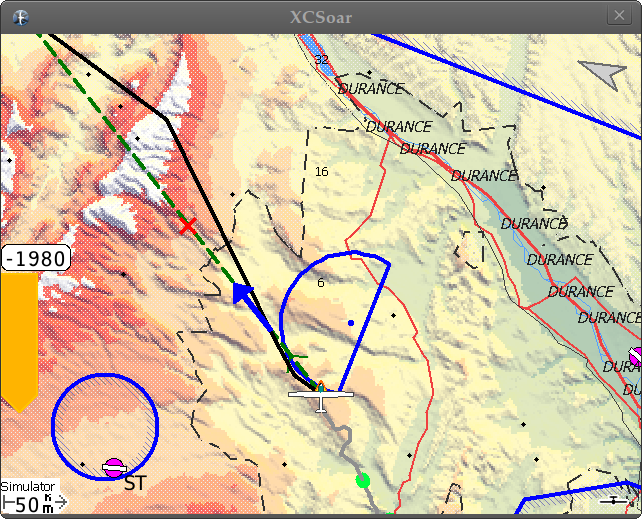
\includegraphics[angle=0,width=1.0\linewidth,keepaspectratio='true']{figures/route3.png}
\end{center}

Le calcul d'optimisation de la route est basé sur la polaire du planeur.
Les routes sont optimisées pour minimiser le temps de vol. Par défaut, le calcul d'optimisation de route est inactif. Il peut être activé pour prendre en compte uniquement
le relief ou le relief et les espaces aériens. \config{routemode}

\begin{description} 
\item[Aucun] Calcul d'optimisation de route inactif.
\item[Relief] La route évitera le relief.
\item[Espace aérien]  La route évitera les espaces aériens.
\item[Les 2] La route évitera les espaces aériens et le relief.
\end{description}

Le relief est survolé en prenant en compte la hauteur minimum par rapport au relief (la garde au sol),\config{safetyterrain}
mais sans prendre en compte de distance minimale latérale.
Une route optimisée peut amener à une hauteur d'arrivée supérieure à la hauteur minimum d'arrivée~: par exemple si l'objectif se trouve juste derrière une montagne abrupte.

Les espaces aériens sont évités horizontalement par une marge d'environ 250~mètres. Il n'y a pas de marge verticale imposée. Des routes valides peuvent passer au-dessus ou au-dessous d'un espace aérien.

Si le calage MacCready est positif, les montées peuvent être permises en option
sur les routes calculées. La hauteur maximale de montée
peut être limitée à 500~m au-dessus du plafond du départ ou de l'objectif,
ou augmentée jusqu'au plafond défini comme plafond des thermiques.
\config{routeceiling} Les montées au-dessus de la plus haute altitude de départ ou de l'objectif sont pénalisées par un taux de montée plus faible que la
valeur réelle du MacCready.

Voici une partie des approximations et limitations du calcul de route~:
\begin{itemize}
\item quand les montées sont nécessaires (et autorisées) pour atteindre le prochain point de virage, les montées sont considérées comme ayant lieu en début de route.
\item les portions de transition en montée sont considérées comme étant à altitude constante, et équivalentes à une série de petites montées réparties le long de la route.
\item le long de la route, les virages de plus de 90° ne sont pas autorisés.
\item si l'algorithme de calcul de route n'aboutit pas, le calcul repasse en mode vol direct depuis la position actuelle du planeur vers l'objectif.
\end{itemize}
